%! Author = Sujal Singh
%! Date = 4/9/24

% Preamble
\documentclass[11pt]{beamer}
\title[Power Plants, Collegiality and Loyalty, \ldots]{%
    \large Case Study: Power Plants, Collegiality and Loyalty, Collective Bargaining, Confidentiality,
    Conflict of Interest
}
\author[Sujal, Divyanshi, Priyanshu \ldots]{%
    \textbf{Group 9:}\\%
    \(|\) Sujal Singh \(|\) Divyanshi Panchal \(|\) Priyanshu Raj \(|\)\\\(|\) Chitransh Koshta \(|\) Prashant
    Pulkit \(|\)%
    \vspace*{-15pt}
}
\date[Chitransh, Prashant]{\textbf{Enrollment Numbers:}\\0\{41-45\}19051723}

\usetheme{Madrid}
\setbeamertemplate{navigation symbols}{}
\setbeamertemplate{frametitle continuation}[from second][]

% Packages
\usepackage{amsmath}
\usepackage{copyrightbox}

% Document
\begin{document}
    \maketitle

    \begin{frame}[t,allowframebreaks]{Case Study: Power Plants}
        \textbf{Three Mile Island Accident}\\[10pt]
        \begin{minipage}[t]{0.45\textwidth}
            \vspace*{-8pt}
            \begin{figure}
                \label{fig:three-mile-island}
                \copyrightbox[b]
                {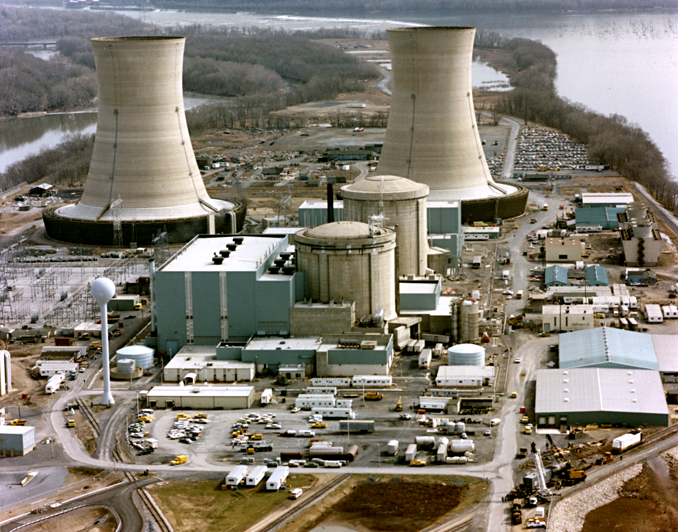
\includegraphics[width=150pt]{images/three-mile-island}}
                {\tiny Source: Wikipedia}
            \end{figure}
        \end{minipage}
        \begin{minipage}[t]{0.54\textwidth}%
            The Three Mile Island Unit 2 (TMI-2) nuclear power plant in Pennsylvania experienced a partial meltdown on
            March 28, 1979 which caused an \alert{increase in radiation level and an explosion within the building},
            there were no casualties.\ The reactor was brought under control after 13.5 hours.
        \end{minipage}

        \framebreak
        Here's a breakdown of what happened:\\[10pt]
        \begin{itemize}
            \small
            \item A malfunction in the demineralizer led to the shutdown of water pumps feeding the reactor core.
            \item Reactor pressure rose, triggering safety measures to insert control rods and stop the fission process.
            \item A pressure relief valve remained open, preventing proper cooling of the reactor core.
            \item Water loss from the core and overheating caused fuel rod damage.
            \item A chemical reaction between steam and reactor components produced hydrogen gas.
        \end{itemize}

        \framebreak

        \textbf{Chernobyl Disaster (\mathbf{1986})}\\[5pt]

        \begin{center}
            \begin{figure}
                \label{fig:chernobyl}
                \copyrightbox[b]
                {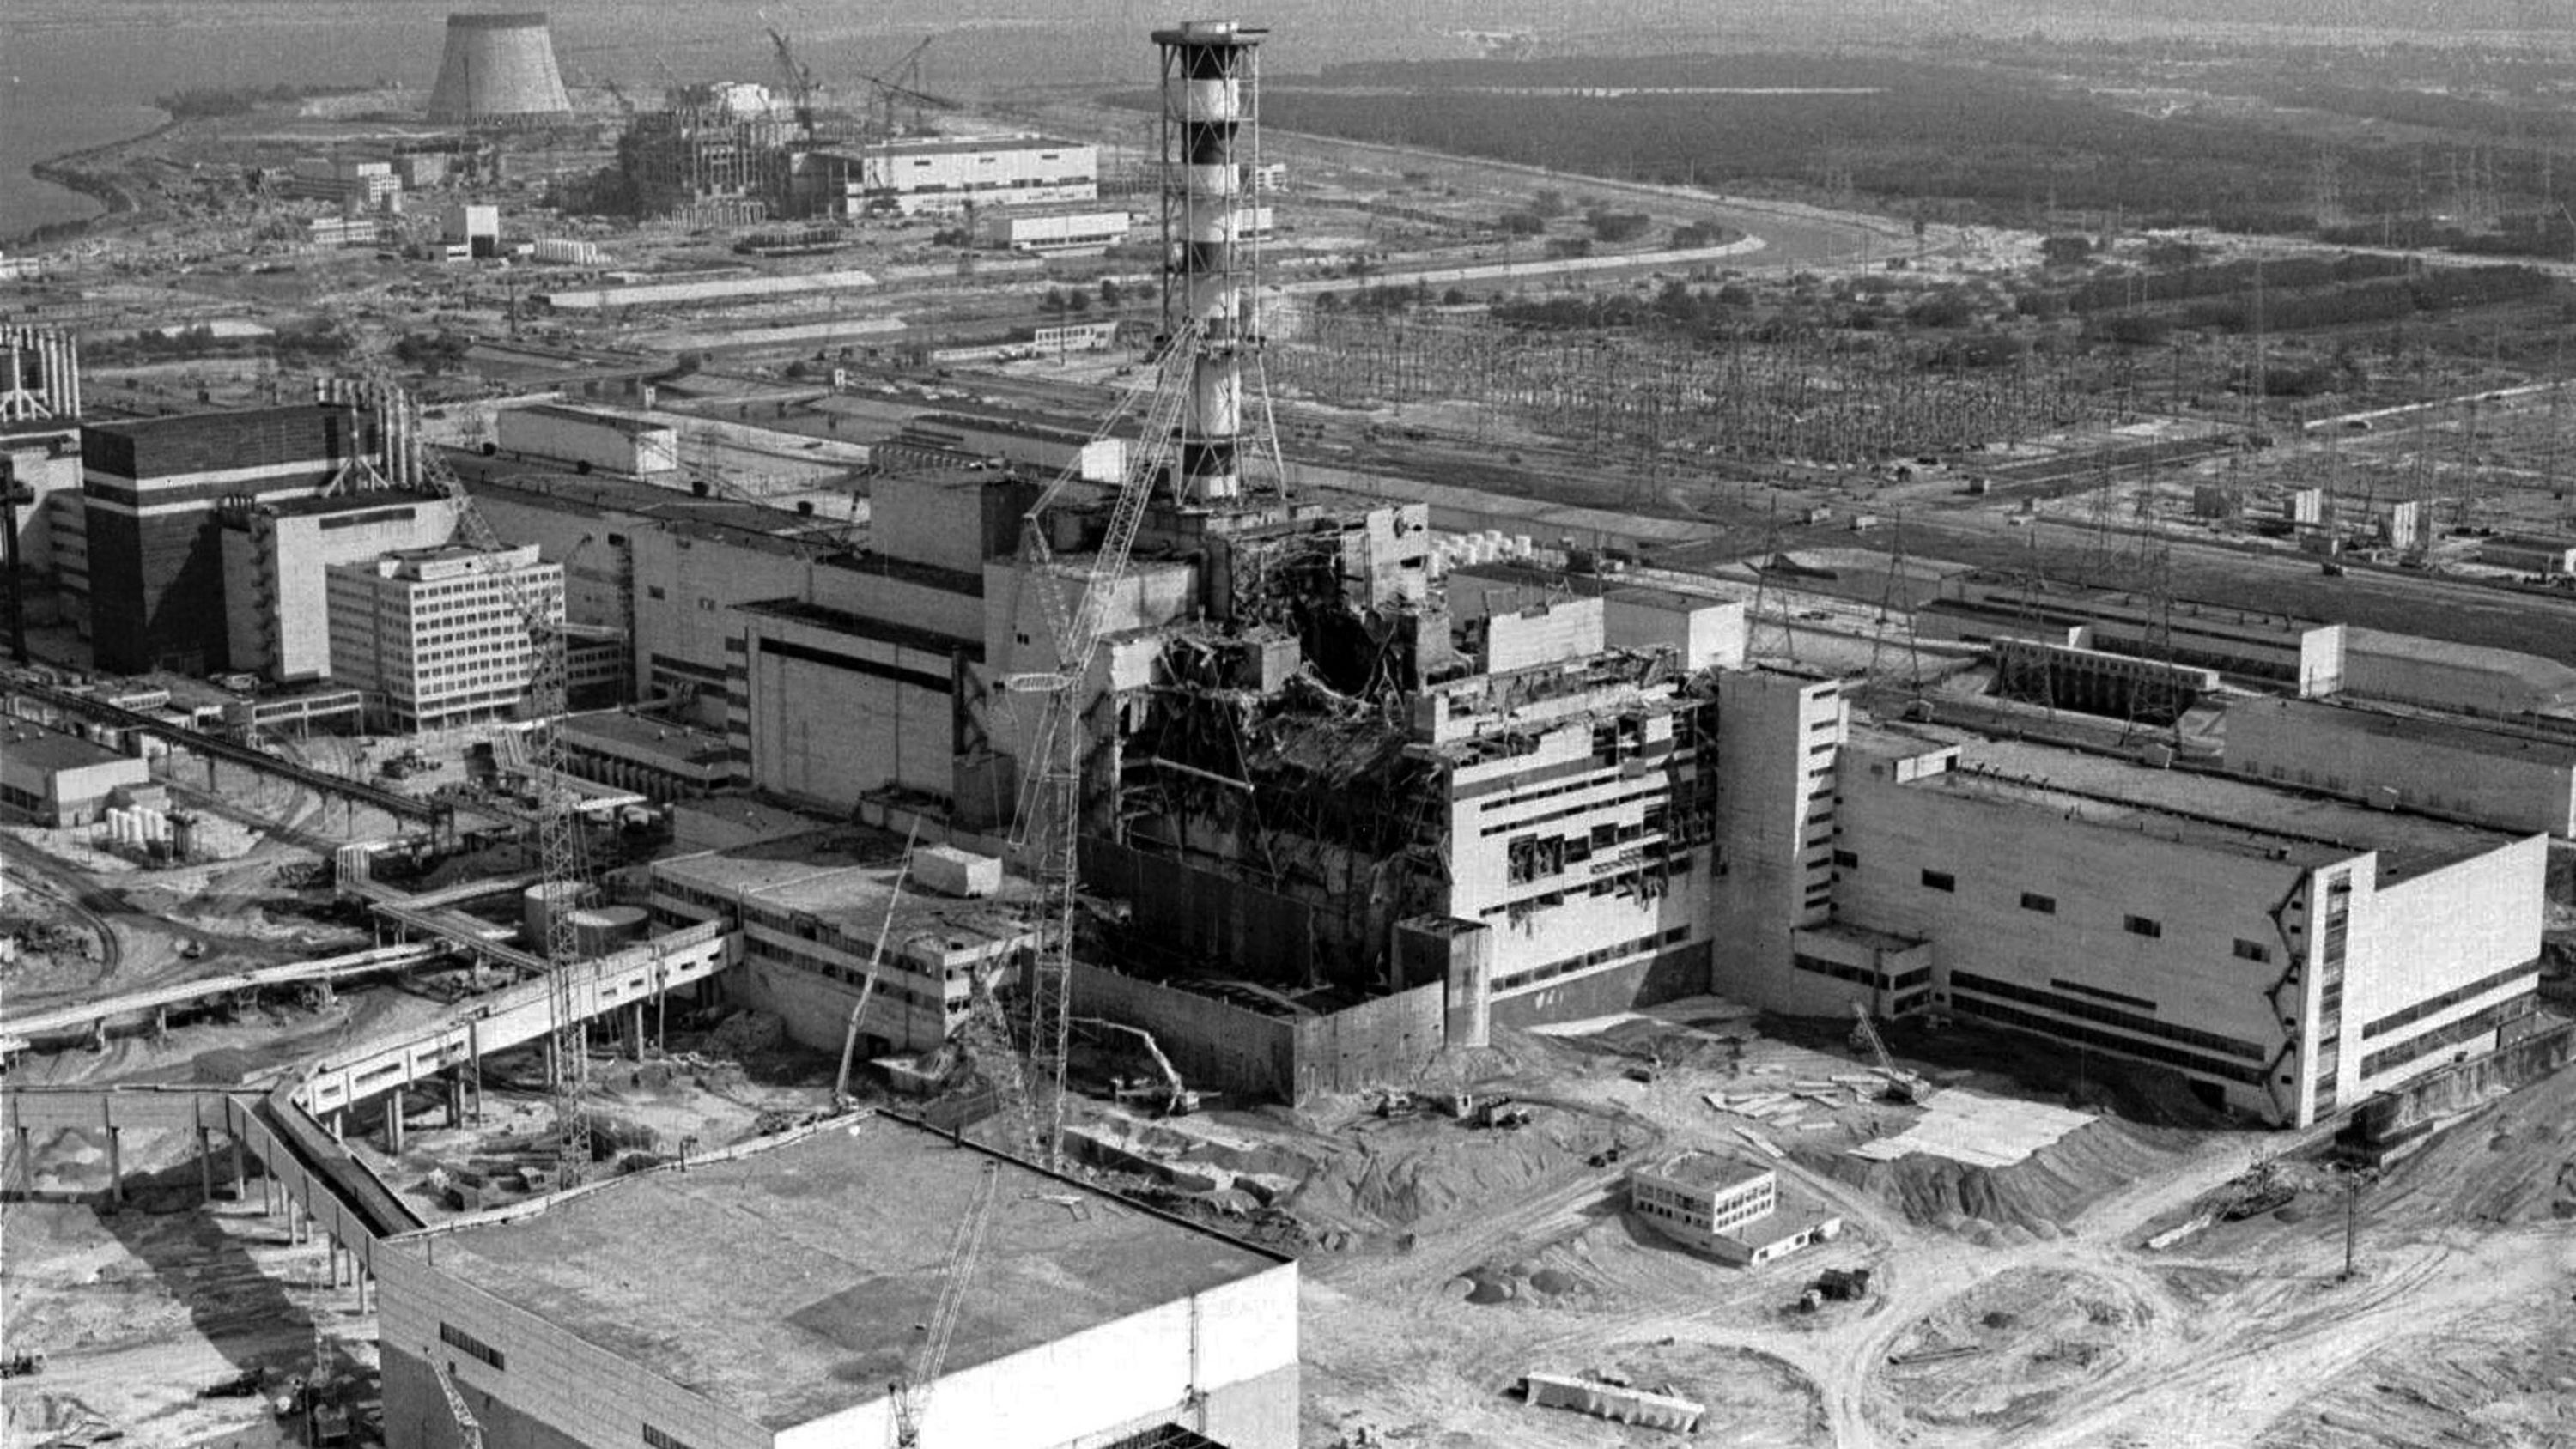
\includegraphics[width=180pt]{images/chernobyl}}
                {\tiny Source: CNN}

            \end{figure}
        \end{center}

        \begin{itemize}
            \item The Chernobyl plant used RBMK reactors, with a graphite water cooling system, known for safety
            vulnerabilities.
            \item A turbine generator test was scheduled during maintenance, requiring a power reduction to 700 MW.
        \end{itemize}

        \begin{itemize}
            \setlength{\leftmarginii}{10pt}
            \item \textbf{Ignoring Safety Measures:}
            \begin{itemize}
                \item Operators disconnected the emergency cooling system.
                \item The test was conducted at an abnormally low power level (200 MW).
                \item Emergency signals and automatic shutdowns were deliberately blocked.
            \end{itemize}
            \item \textbf{Operator Error and Escalation}
            \begin{itemize}
                \item Operators further compromised safety by raising control rods to increase power, causing a rise
                in reactor temperature and fission rate.
            \end{itemize}
            \item \textbf{Catastrophic Outcome}
            \begin{itemize}
                \item The reactor core melted, leading to a fire and the release of radioactive materials across the
                USSR and Europe.
                \item Evacuation of nearby residents was delayed for hours after the explosion.
            \end{itemize}
            \item \textbf{Casualties and Impact}
            \begin{itemize}
                \item Over 30 plant workers died, with 200 suffering burns.
                \item Long-term health effects resulted in an estimated 8,000 deaths.
                \item Agricultural production was significantly impacted by radioactive contamination for years.
            \end{itemize}
        \end{itemize}
        \\[5pt]
        \textbf{Safety Lessons from TMI and Chernobyl}
        \begin{itemize}
            \item Stronger containment structures to prevent radiation leaks after explosions.
            \item If power increases during critical tests, like at Chernobyl, should be rejected or halted entirely
            with safety systems reactivate
            \item Continuous monitoring of critical components is essential for early detection of issues.
            \item Establish comprehensive emergency plans.
            \item Prompt notification of superiors and timely evacuation of nearby residents (both TMI and Chernobyl).
        \end{itemize}
    \end{frame}

    \begin{frame}[t]{Collegiality and Loyalty}
    \end{frame}

    \begin{frame}[t]{Collective Bargaining}
    \end{frame}

    \begin{frame}[t]{Confidentiality}
    \end{frame}

    \begin{frame}[t]{Conflict of Interest}
    \end{frame}
\end{document}